\subsection{Confocal of RNA-binding mutant}
\subsubsection{i2f-24}
\myparagraph{hi2f24}
some text

\begin{figure}
    \centering
    
\includegraphics[width=0.5\linewidth]{10. Chapter 5//Figs//04. IFIT2-mutant confocal/00. placeholder.png}
    \caption[hi2f24]{hi2f24}
    \label{hi2f24}
\end{figure}

\myparagraph{bi2f24}
Cell Line: VERO
Treatment: bIFIT2-FLAG-RBM
Detecting magenta: exogenous bovine IFIT2 RBM
Detecting cyan: background

Exogenous bovine IFIT2 RNA-binding mutant (RBM) seems to have the same distribution and effect on the cell as human IFIT2-FLAG overexpression.

\begin{figure}
    \centering
    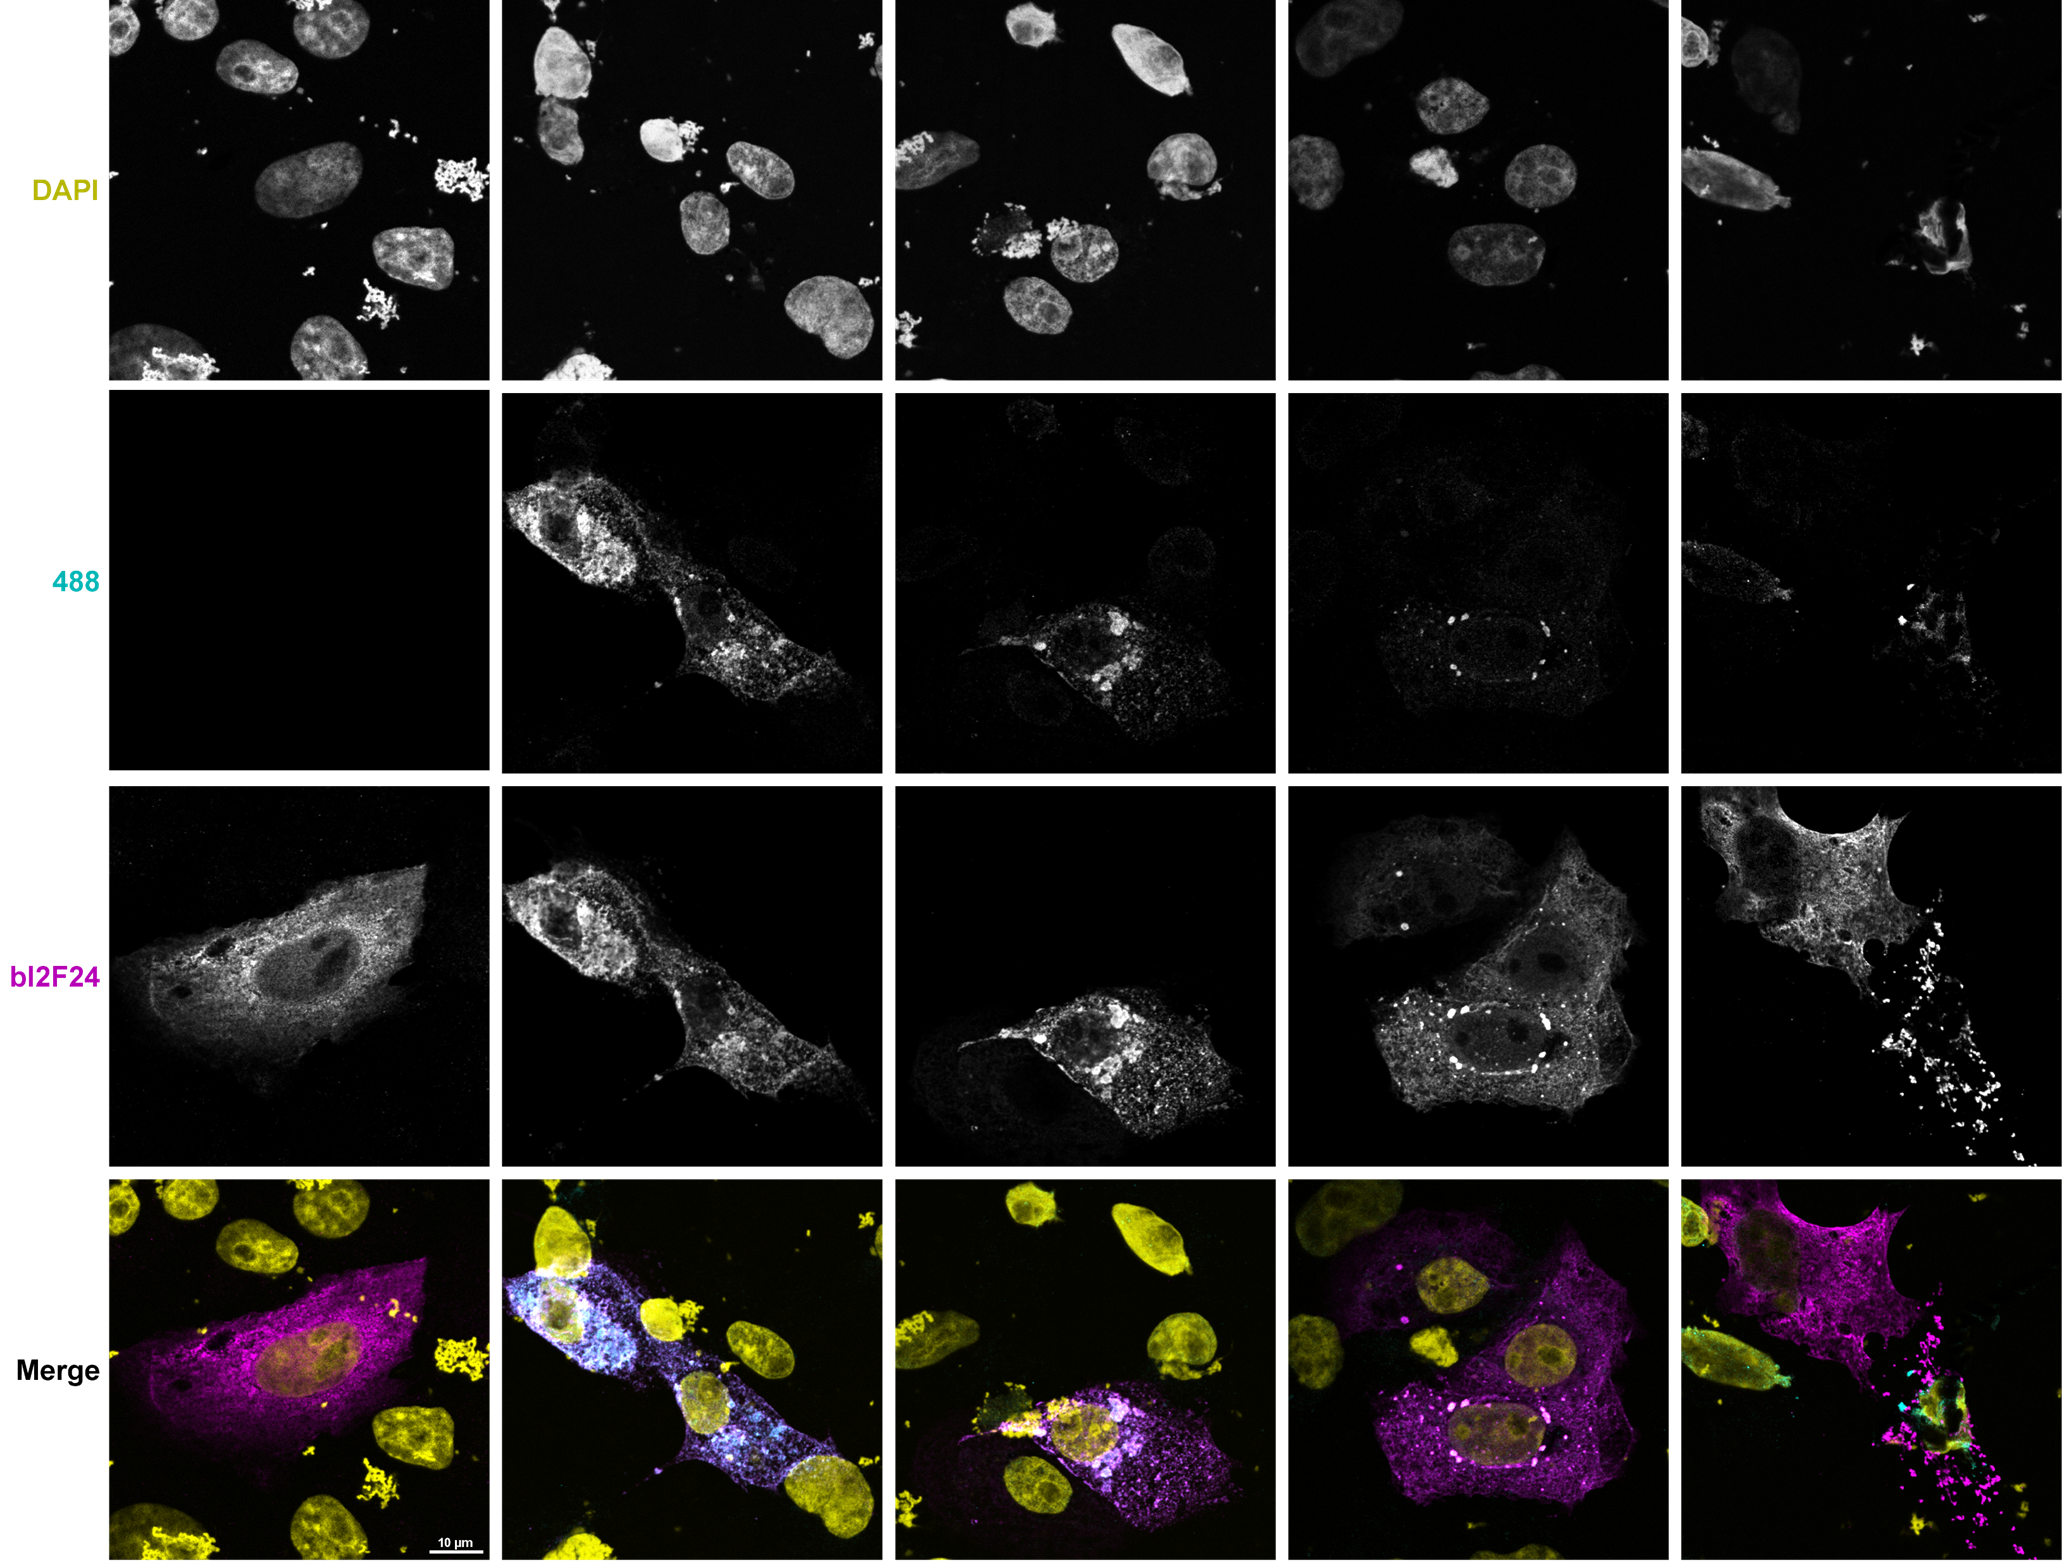
\includegraphics[width=1\linewidth]{10. Chapter 5/Figs/04. IFIT2-mutant confocal/01. bi2f24.png}
    \caption[bi2f24]{bi2f24}
    \label{bi2f24}
\end{figure}

\subsubsection{pIB}
\myparagraph{hi2f24 + hnhp}
some text

\begin{figure}
    \centering
    
\includegraphics[width=0.5\linewidth]{10. Chapter 5//Figs//04. IFIT2-mutant confocal/00. placeholder.png}
    \caption[hi2f24 + hnhp]{hi2f24 + hnhp}
    \label{hi2f24 + hnhp}
\end{figure}


\myparagraph{hi2f24 + bnbp}
some text

\begin{figure}
    \centering
    
\includegraphics[width=0.5\linewidth]{10. Chapter 5//Figs//04. IFIT2-mutant confocal/00. placeholder.png}
    \caption[hi2f24 + bnbp]{hi2f24 + bnbp}
    \label{hi2f24 + bnbp}
\end{figure}

\myparagraph{bi2f24 + hnhp}
Cell Line: VERO
Treatment: hNhP + bIFIT2-FLAG-RBM
Detecting magenta: exogenous bovine IFIT2 RBM
Detecting cyan: human pIB

In the second experiment we see consistent colocalization and/or inclusion of bovine IFIT2 RNA-binding mutant with human pseudo inclusion bodies.

\begin{figure}
    \centering
    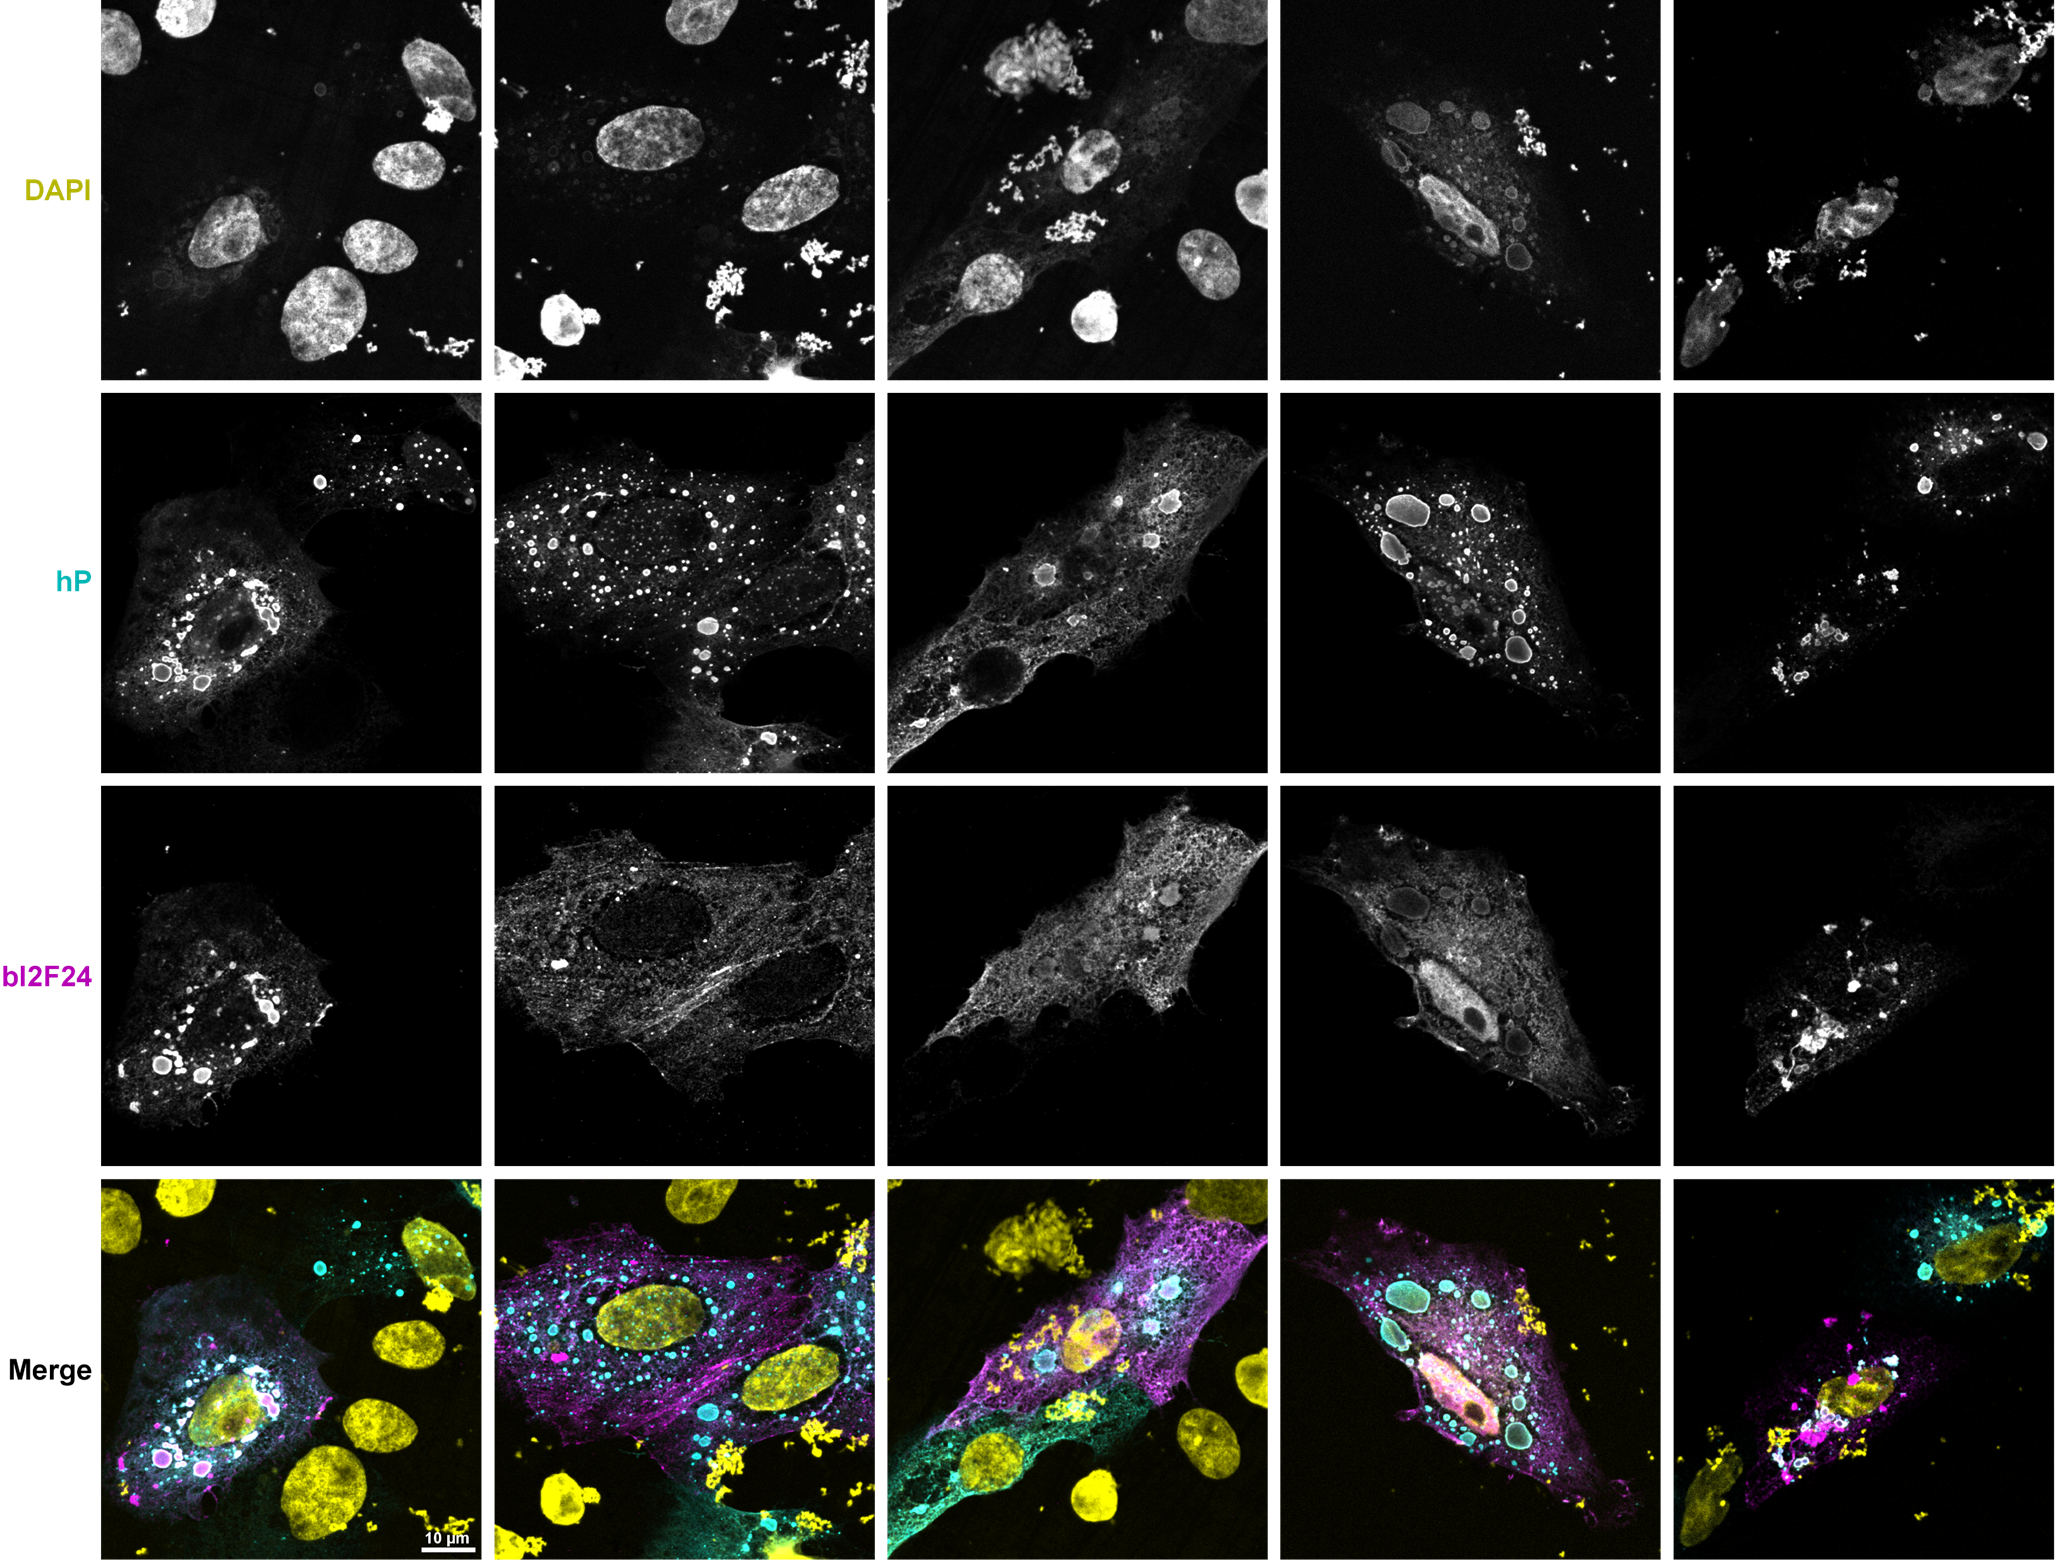
\includegraphics[width=0.5\linewidth]{10. Chapter 5/Figs/04. IFIT2-mutant confocal/02. bi2f hnhp.png}
    \caption[bi2f24 + hnhp]{bi2f24 + hnhp}
    \label{bi2f24 + hnhp}
\end{figure}

\myparagraph{bi2f24 + bnbp}
some text

\begin{figure}
    \centering
    
\includegraphics[width=0.5\linewidth]{10. Chapter 5//Figs//04. IFIT2-mutant confocal/00. placeholder.png}
    \caption[bi2f24 + bnbp]{bi2f24 + bnbp}
    \label{bi2f24 + bnbp}
\end{figure}


\subsubsection{Infection transfection}
\myparagraph{hi2f24 + hrsv}
some text

\begin{figure}
    \centering
    
\includegraphics[width=0.5\linewidth]{10. Chapter 5//Figs//04. IFIT2-mutant confocal/00. placeholder.png}
    \caption[hi2f24 + hrsv]{hi2f24 + hrsv}
    \label{hi2f24 + hrsv}
\end{figure}


\myparagraph{hi2f24 + brsv}
some text

\begin{figure}
    \centering
    
\includegraphics[width=0.5\linewidth]{10. Chapter 5//Figs//04. IFIT2-mutant confocal/00. placeholder.png}
    \caption[hi2f24 + brsv]{hi2f24 + brsv}
    \label{hi2f24 + brsv}
\end{figure}

\myparagraph{bi2f24 + hrsv}
some text

\begin{figure}
    \centering
    
\includegraphics[width=0.5\linewidth]{10. Chapter 5//Figs//04. IFIT2-mutant confocal/00. placeholder.png}
    \caption[bi2f24 + hrsv]{bi2f24 + hrsv}
    \label{bi2f24 + hrsv}
\end{figure}

\myparagraph{bi2f24 + brsv}
some text

\begin{figure}
    \centering
    
\includegraphics[width=0.5\linewidth]{10. Chapter 5//Figs//04. IFIT2-mutant confocal/00. placeholder.png}
    \caption[bi2f24 + brsv]{bi2f24 + brsv}
    \label{bi2f24 + brsv}
\end{figure}

\subsubsection{Summary}
We have described how bovine IFIT2 RNA-binding mutant was designed based on the published human IFIT2 RNA-binding mutant data (needs to be annotated more). Overexpression of bovine IFIT2 RNA-binding mutant yields cellular distribution and morphology similar to what was observed with overexpressing human IFIT2-FLAG, suggesting that the mutant proteins are not toxic to the cells. In the first experiment where we were looking at interaction between bovine IFIT2 RNA-binding mutant and human pseudo inclusion bodies we saw several phenotypes. We observed bovine IFIT2 RNA-binding mutant being excluded from small and big pIBs and pIB associated filamentous network, while fully or partially colocalising with other pIBs. In a subsequent experiment we observed only colocalization and inclusion formation. When assessing the interaction between bovine IFIT2 RNA-binding mutant and human pIBs formed using wild-type human RSV P and GFP-tagged human RSV N, we observed consistently in two experiments that bovine IFIT2 RNA-binding mutant colocalises to the pIB structures.